Our approach, depicted in Figure~\ref{fig:overview}, consists of three parts: a) an image acquisition process based on the z-stacking technique; b) a method for assessing the quality of images that explores frequency domain features and basic statistical analysis tools and outputs a quantitative index that allows the selection of focused images and c) an image fusion procedure, based on the Laplacian of Gaussian filter and energy of edges, which forms the final image. \autoref{fig:overview}.(a) denotes the image acquisition process, which consists of collecting specimens of plants, acquiring images with microscopes and organizing the datasets. Then the images undergo our IQA method in Figure~\ref{fig:overview}.(b), and a subset of the images is selected for registration by means of statistical methods. Finally, Figure~\ref{fig:overview}.(c) represents the image fusion procedure, which aims to produce a high-quality image.

\begin{figure}[ht]
  \centering
  \caption{Overview of each stage of our approach: \textbf{(a)} image acquisition and registration, \textbf{(b)} selection of images after IQA and \textbf{(c)} image fusion.}
  \label{fig:overview}
  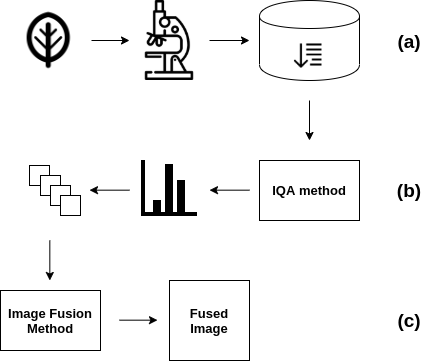
\includegraphics[scale=0.8]{images/overview.png}
  \centering
  \fautor
\end{figure}